%
% 2023/11/1
%
%
%

\documentclass[varwidth=12cm,border=1cm,tikz]{standalone}
% https://latexdraw.com/plot-a-function-and-data-in-latex/
 \usepackage[ipaex]{luatexja-preset} % standaloneとlualatexjaを共存させる方法?
\usepackage{tikz}
\usepackage{pgfplots}
\usepackage{physics}

\pgfplotsset{compat = newest}
 % axis style, ticks, etc
 \pgfplotsset{every axis/.append style={
                    label style={font=\Huge}, % ラベルだけ大きく
                    title style={font=\huge},
                    tick label style={font=\huge},
                    legend style={font=\huge},
                    }}
 \usepgfplotslibrary{colorbrewer}
 \usetikzlibrary{pgfplots.colorbrewer}
\usetikzlibrary{arrows.meta,backgrounds}
\tikzset{white background/.style={show background rectangle,tight background,
background rectangle/.style={fill=white}}}

\begin{document}

\def\eps0{50000}
\def\epsinf{0.2}
\def\gamma{100}
\def\freq0{500}

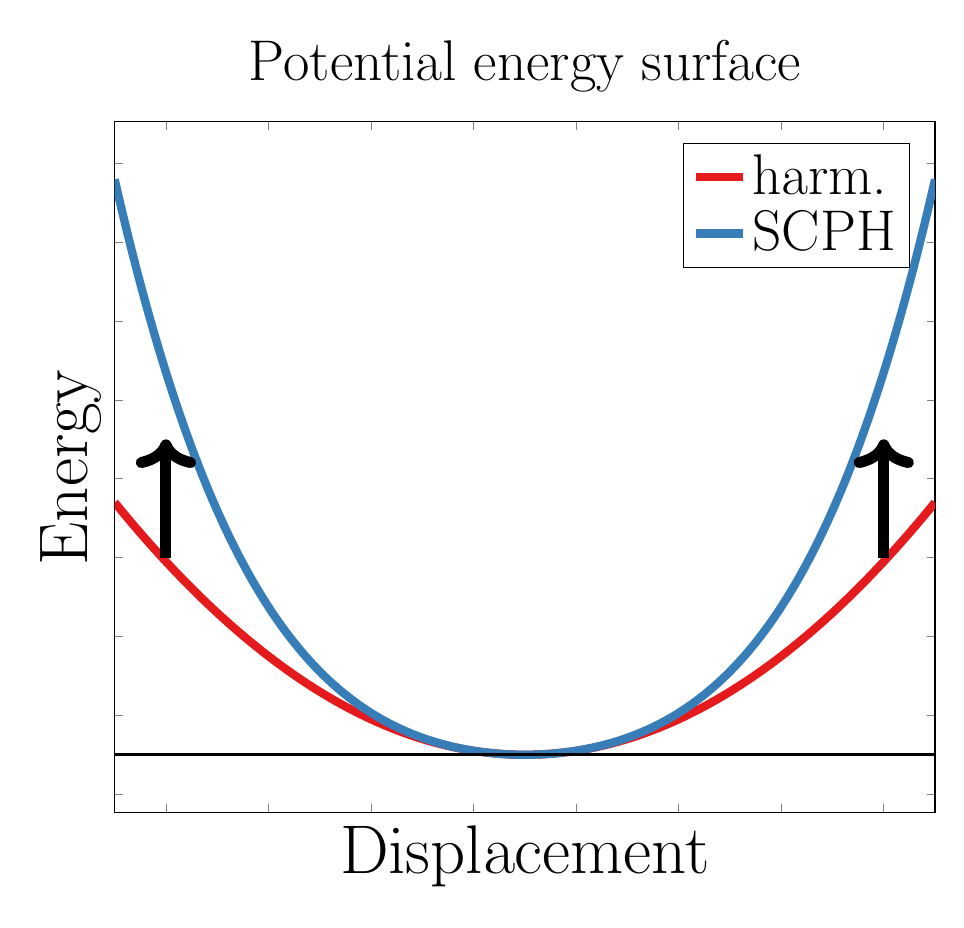
\begin{tikzpicture}[white background]
     \tikzset{every node}=[font=\Large]
        % axis環境が2次元plot
        \begin{axis}[ %グラフ設定
            xmin = -8, xmax = 8,
            % ymin = -0.003, ymax = 0.010,
            ticks=none,
	    xlabel=$\mathrm{Displacement}$,
	    ylabel=$\mathrm{Energy}$,
	    title=Potential energy surface,
            % grid = both,
            minor tick num = 1,
            major grid style = {lightgray},
            minor grid style = {lightgray!25},
            width = 12cm, %\textwidth,
            % height = 0.75\textwidth,
            legend cell align = {left},
            legend pos = north east
        ]
            %\coordinate (A) at (80,-1); 

	    %\coordinate (B) at (80,5);
	 
	 
	 % x*x
	 \addplot[domain = -8:8,samples=1000,line width=3,Set1-A] {0.5*x*x}; % \epsinf+(\eps0-\epsinf)*(\freq0*\freq0-x*x)/((\freq0*\freq0-x*x)*(\freq0*\freq0-x*x)+\gamma*\gamma*x*x)};
	 \addplot[domain = -8:8,samples=1000,line width=3,Set1-B] {0.5*x*x+0.01*x*x*x*x}; % \epsinf+(\eps0-\epsinf)*(\freq0*\freq0-x*x)/((\freq0*\freq0-x*x)*(\freq0*\freq0-x*x)+\gamma*\gamma*x*x)};

	 \addplot[->,black,line width =4, mark=none]coordinates {(7, 25) (7, 40)};
	 \addplot[->,black,line width =4, mark=none]coordinates {(-7, 25) (-7, 40)};
         \addplot[black,solid, line width = 1, mark=none] coordinates {(-8,0) (8,0)};


%            \addplot[blue,solid, line width = 2, mark = none] table [x index=2, y index=4] {\au};
%            \addplot[red ,solid, line width = 2, mark = none] table [x index=2, y index=4] {\eu};
	    % \addplot[blue, dotted, line width = 2, mark=none] coordinates {(80,-1) (80,5)}; 
	    % \addplot[orange, dotted, line width = 2, mark=none] coordinates {(\freq0,-0.002) (\freq0,0.01)};  % !! これはつかっても良いもか
%	    \addplot[blue,dotted, line width = 2, mark=none] coordinates {(598,0) (598,180)};
            %\addplot[red, only marks] table [x ={x}, y = {y2}] {\table};
            %\addplot[teal, only marks, mark = x, mark size = 3pt]
            %    table [x = {x}, y = {y3}] {\table};
	    % \node[] at (\freq0,-0.001) {$\omega_0$}; % !! これは使ってもいいかも.
	    % \node[] at (170,-0.5) {$\omega_0+\Delta\omega$};
	    % \node[] at (90,2) {$\gamma$};
            \legend{
	       harm.,
	       SCPH
	    }
	    %,
            %    Plot only with marks,
            %    Plot with other type of marks}
        \end{axis}
    \end{tikzpicture}
\end{document}

% \documentclass{standalone}

% \usepackage{tikz}
% \usepackage{pgfplots}

% \pgfplotsset{compat = newest}

% \begin{document}
%     \begin{tikzpicture}
%         \begin{axis}[
%             xmin = 0, xmax = 30,
%             ymin = -1.5, ymax = 2.0,
%             xtick distance = 2.5,
%             ytick distance = 0.5,
%             grid = both,
%             minor tick num = 1,
%             major grid style = {lightgray},
%             minor grid style = {lightgray!25},
%             width = \textwidth,
%             height = 0.5\textwidth,
%             xlabel = {$x$},
%             ylabel = {$y$},
%             legend cell align = {left},
%         ]
%             \addplot[
%                 domain = 0:30,
%                 samples = 200,
%                 smooth,
%                 thick,
%                 blue,
%             ] {exp(-x/10)*( cos(deg(x)) + sin(deg(x))/10 )};
            
%             \addplot[
%                 smooth,
%                 thin,
%                 red,
%                 dashed
%             ] file[skip first] {cosine.dat};
            
%             \legend{Plot from expression, Plot from file}
%         \end{axis}
%     \end{tikzpicture}
% \end{document}